\subsection{Backbone and activation}
The backbone is CSPDarknet53\cite{CSPDarknet53}, most notably used in YOLOv4\cite{yolov4}. This backbone obtained better result than the CSPResNeXt-50\cite{resNeXt} in the YOLO paper, which is why it is used. Inspiration could also be taken from Zhuang \textit{et al.}\cite{zhuang2019}, with passthrough and concatenation from earlier layers.

\begin{figure}[H]
  \centering
  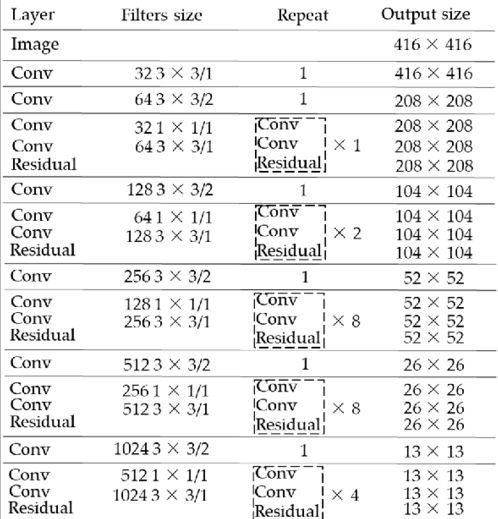
\includegraphics[width=\textwidth]{darknet53Archi.png}
	\caption[]{Architecture of the darknet 53 backbone.}
  \label{}
\end{figure}

The choice of a activation function would need to be tested. Mish\cite{mish}(Figure~\ref{fig:mish}) and Swish (Figure~\ref{fig:swish}) or even Scaled Exponential Linear Unit (SELU) (Figure~\ref{fig:selu}) are good candidates. 

\begin{figure}[H]
	\begin{subfigure}[t]{.3\textwidth}
		  \centering
		  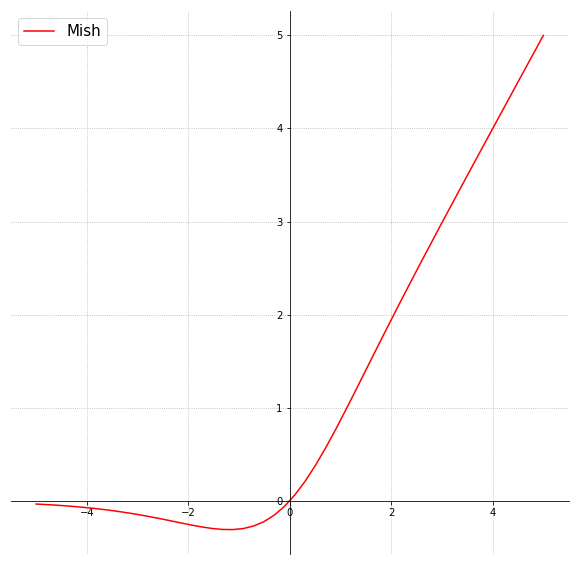
\includegraphics[width=\linewidth]{mish}  
		  \caption{Mish Activation Function}
		  \label{fig:mish}
	\end{subfigure}
	\begin{subfigure}[t]{.3\textwidth}
		  \centering
		    % include second image
		      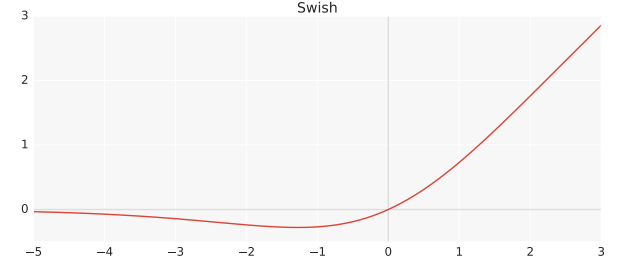
\includegraphics[width=\linewidth]{swish}  
		        \caption{Swish Activation Function}
			  \label{fig:swish}
	\end{subfigure}
	\begin{subfigure}[t]{.3\textwidth}
		\centering
		% include second image
		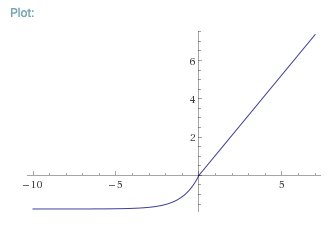
\includegraphics[width=\linewidth]{selu}  
		\caption{Scaled Exponential Linear Unit (SELU) Activation Function}
		\label{fig:selu}
	\end{subfigure}
	\caption{Activation Function Candidates}
	\label{fig:activations}
\end{figure}


\subsection{Dual Scale Detectors}
An idea introduced in YOLT\cite{yolt} is to use two different detectors running simultaneously: one trained on small scale images to detect small objects, the other trained on larger images to detect bigger objects. The small scale network would be fed small chips of images, while the large scale network would be fed downscaled large swathes of terrain. This meant that the large scale network would run much less often than the small scale network, and mitigate the loss of performance of running two network at the same time.

An ensemble method similar to this could be used, where two networks try to find objects at different scales.

\subsection{Multi-scale Feature Fusion}
To be able to detect the small objects often seen in LiDAR data, a multi-scale feature fusion module needs to be used. There are a few existing modules and techniques that can boost the detection rates of a model by aggregating low level feature maps from earlier layers with ones from higher layers. We call those modules Multi Layer Feature Fusion (MLFF). 

The MLFF module from Zhuang \textit{et al.}\cite{zhuang2019} takes 3 feature maps from different layers, upscales and concatenates them, then applies a series of convolution operations to obtain 3 predictions at different scale.

\begin{figure}[H]
  \centering
  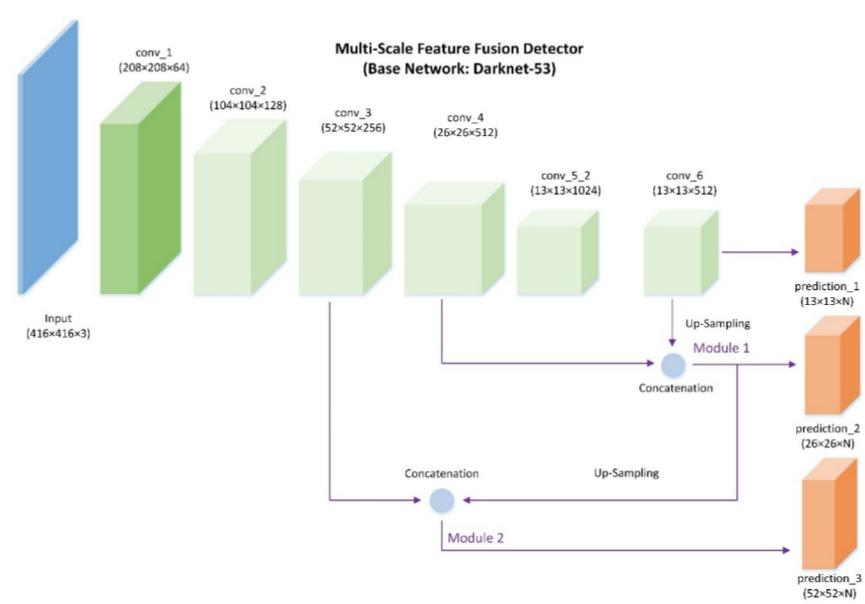
\includegraphics[width=\textwidth]{msFusionDetectorArchi}
	\caption[]{Feature Fusion implementation of Zhuang \textit{et al.}. We are only interested in the bottom part of the figure, with feature maps from different levels being concatenated.}
  \label{fig:mlffZhuang}
\end{figure}

The MLFF module from Qian \textit{et al.}\cite{qianAl} shown in Figure~\ref{fig:mlffQian} takes each proposal generated by a Region Proposal Networks, and maps its position to all level of feature map generated by the Feature Proposal Networks. From there it obtains $N$ regions of the feature maps ($N$ being the number of levels), which it transforms into $7 \times 7$ feature maps through the RoiAlign\cite{maskRCNN} operation. Finally, it concatenates these 4 regions along the channel dimensions, and applies two convolution operations along with a Fully Connected Layer for bounding box regression and classification.

\begin{figure}[H]
  \centering
  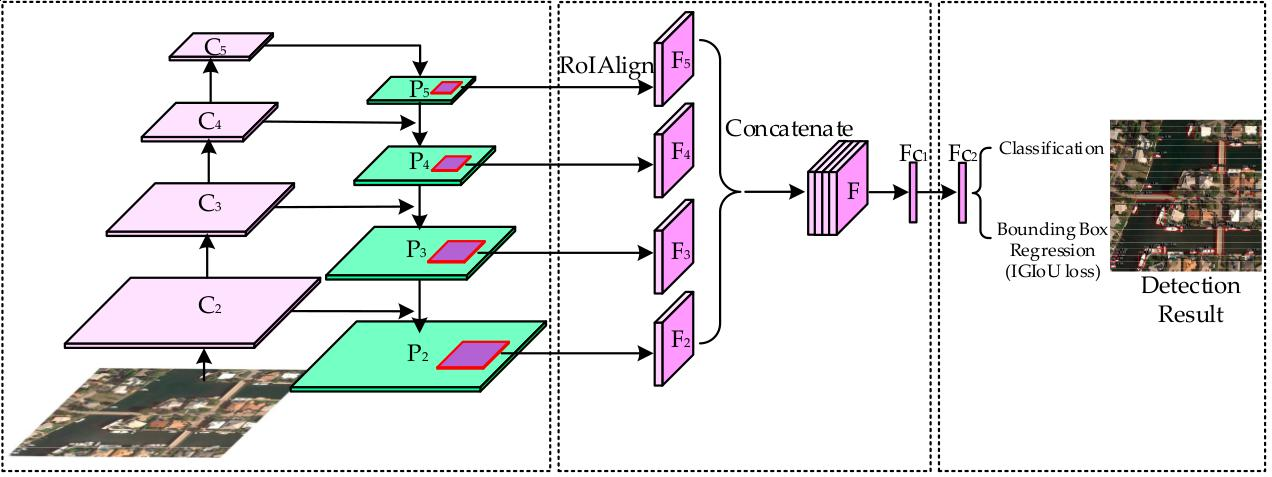
\includegraphics[width=\textwidth]{ODRSIArchi}
	\caption[]{Architecture of the model from Qian et al. We are interested in the module shown in (b), where particular regions of different feature maps are concatenated together}
  \label{fig:mlffQian}
\end{figure}

The Path Aggregation Network is a sort of multi layer feature fusion module. Following the same principle as the MLFF from Qian \textit{et al.}, PAN takes the features maps generated by a Feature Proposal Networks. It first downscales the lower level layer (denoted $P_i$ with a $3 \times 3$ convolution operation with a stride of 2. It then adds element wise this downscaled layer with the layer $P_{i+1}$. This is done iteratively until the up most layer is attained. \textbf{In the YOLOv4 paper, instead of adding the layers, a concatenation is done}.

\begin{figure}[H]
     \centering
     \begin{subfigure}[b]{0.3\textwidth}
         \centering
         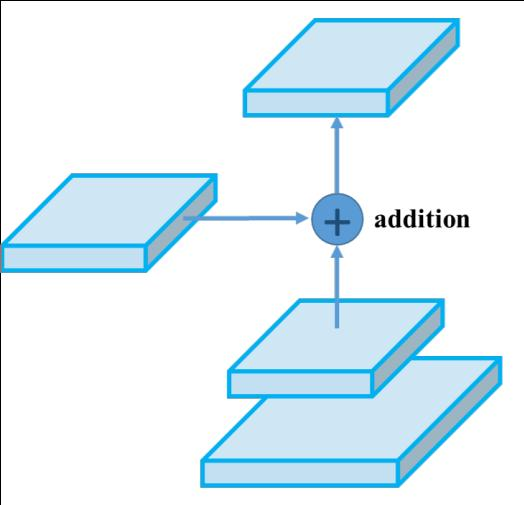
\includegraphics[width=\textwidth]{pan}
         \caption{PAN}
         \label{fig:pan}
     \end{subfigure}
     \begin{subfigure}[b]{0.3\textwidth}
         \centering
         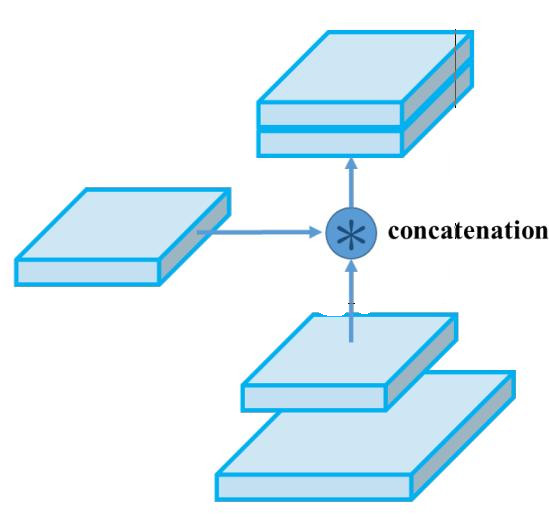
\includegraphics[width=\textwidth]{panMod}
         \caption{Modified PAN}
         \label{fig:panmod}
     \end{subfigure}
   \caption{PAN and its YOLO modification}
   \label{fig:PAN}
\end{figure}

\subsection{Receptive Field Improvements}
To improve the size of the receptive field, the modified SPP module from YOLOv3\cite{yolov3} would be used. Experimentations could be done using dilated convolutions, as seen in Yu \textit{et al.}\cite{yu2015} and Ju \textit{et al.}. Dilated convolution improve the receptive field by increasing the kernel size without increasing the number of parameters in the kernel. This can help reducing the number of parameters, improving performance of the network in terms of Frames Per Seconds. We can replace some of the classical convolution blocks from the CSPDarknet53 backbone with dilated convolution modules, as can be seen in Figure~\ref{fig:dilConvDarknet}. 

\begin{figure}[H]
  \centering
  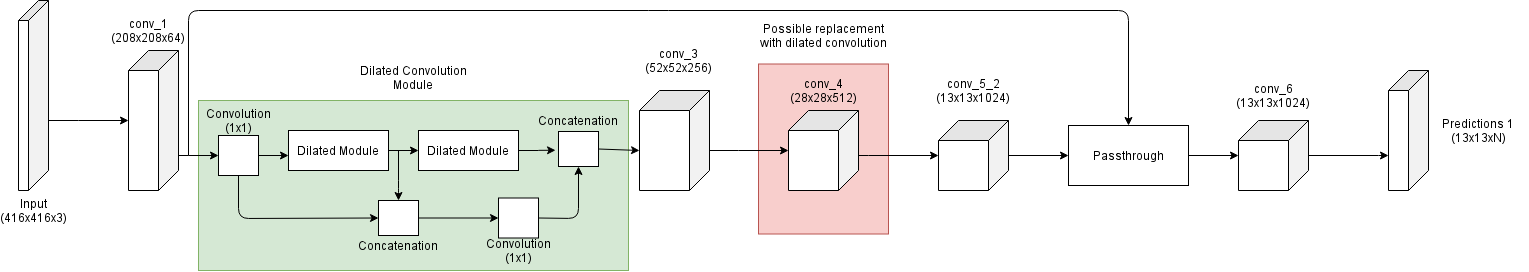
\includegraphics[width=\textwidth]{archiDilConv}
	\caption[]{General Architecture of the Darknet Backbone with a dilated convolution module replacing a convolution block}
  \label{fig:dilConvDarknet}
\end{figure}

\subsection{Attention Modules}
Attention modules are used to improve the accuracy of detections network by increasing the importance of particular regions or channels. The Spatial Attention Module\cite{sam} would be used, as it increases the accuracy without significantly impacting inference speed. Testing would have to be done to evaluate whether the SAM improvement done by Bochkovsky \textit{et al.} in the YOLOv4 paper\cite{yolov4} gives a performance increase.

\begin{figure}[H]
     \centering
     \begin{subfigure}[b]{0.4\textwidth}
         \centering
         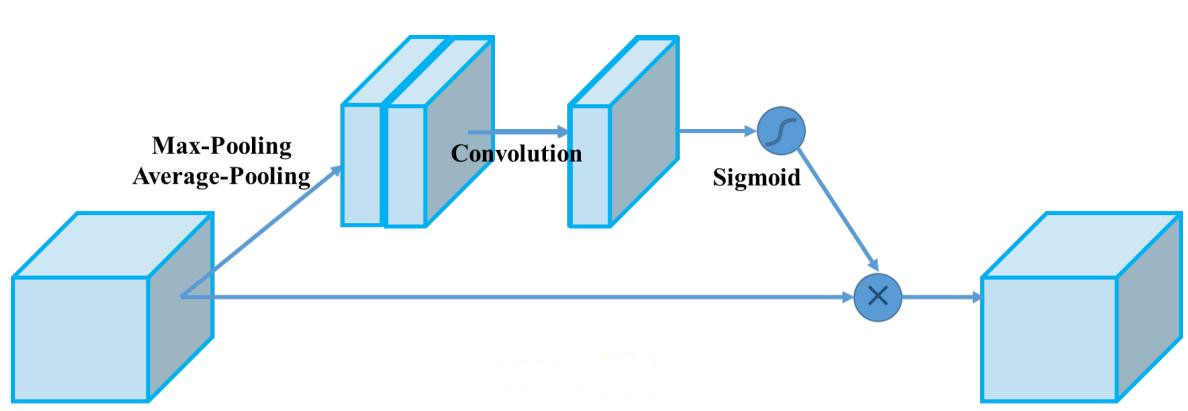
\includegraphics[width=\textwidth]{sam}
         \caption{SAM}
         \label{fig:samnorm}
     \end{subfigure}
     \begin{subfigure}[b]{0.4\textwidth}
         \centering
         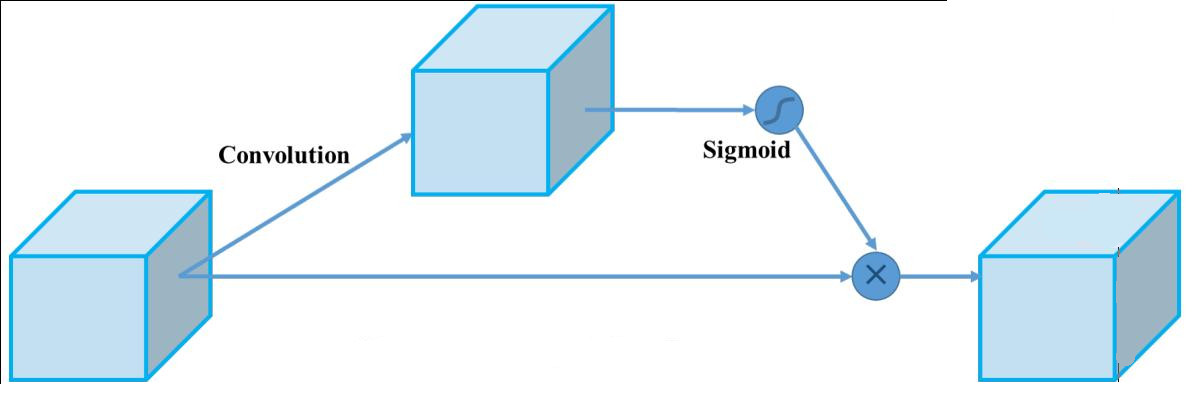
\includegraphics[width=\textwidth]{samMod}
         \caption{Modified SAM}
         \label{fig:samod}
     \end{subfigure}
   \caption{SAM and its YOLO modification}
  \label{fig:SAM}
\end{figure}

\subsection{Post-processing}
Non maximal suppression needs to be used to remove the superfluous bounding boxes generated by the network. Soft Non maximum suppression, as introduced by Qian \textit{et al.} \cite{qianAl} would be used to achieve such a task, while trying to not miss the smaller objects.


\subsection{List of all the possible testing arrangements}
We will need to test a multiple of different modifications on the base CSPDarknet-53 and test out if those modifications results in performances improvements.
\begin{itemize}
	\item Double YOLOv4 trained on large and small scale (similar to YOLT\cite{yolt})
	\item CSPDarknet with one or two dilated convolution modules
	\item MLFF module from Zhuang \textit{et al.}: see Figure~\ref{fig:mlffZhuang}
	\item MLFF module from Qian \textit{et al.}: see Figure~\ref{fig:mlffQian}
	\item Modified PAN module: see Figure~\ref{fig:PAN}
	\item Modified SAM Module: see Figure~\ref{fig:SAM}
	\item Different activations: ReLU, Leaky ReLU, SELU, Mish or Swish
\end{itemize}

